% This is samplepaper.tex, a sample chapter demonstrating the
% LLNCS macro package for Springer Computer Science proceedings;
% Version 2.20 of 2017/10/04
%
\documentclass[runningheads]{llncs}

\usepackage[a4paper]{geometry}
%
\usepackage{graphicx}
\usepackage{minted}
\setminted[bash]{
frame=lines,
breaklines,
fontsize=\footnotesize,
framesep=2mm
}

% Used for displaying a sample figure. If possible, figure files should
% be included in EPS format.
%
% If you use the hyperref package, please uncomment the following line
% to display URLs in blue roman font according to Springer's eBook style:
% \renewcommand\UrlFont{\color{blue}\rmfamily}

\begin{document}
%
\title{Trabalho Prático Nº1 - Processadores e Filtros de Texto}
%
%\titlerunning{Abbreviated paper title}
% If the paper title is too long for the running head, you can set
% an abbreviated paper title here
%
\author{Marco Sousa\inst{1,2}\orcidID{62608} \and
José Malheiro\inst{1,2}\orcidID{93271} \and
Miguel Fernandes\inst{1,2}\orcidID{94269}}
%
\institute{Universidade do Minho\\
\and Licenciatura em Engenharia Informática, Braga, Portugal}
%
%Colocar Numero do Grupo
\maketitle              % typeset the header of the contribution
%
\begin{abstract}
A utilização de expressão regulares permite definir e captar padrões em
streams de texto. No âmbito da discplina de Processamento de Linguagens
será desenvolvido um pograma em Python que vista o uso de Expressões regulares
de maneira a sistematizar a leitura de um dataset do tipo csv e a partir deste gerar um 
conjunto de indicadores estatísticos.

\keywords{Expressões regulares \and Python \and HTML \and CSV.}
\end{abstract}
%
%
%
\section{Introdução}
\subsection{Contextualização} 

O presente relatório foi escrito no âmbito da Unidade Curricular (UC) de Processamento de Linguagens (PL), apresentando 
como objetivo a descrição da solução desenvolvida para o primeiro trabalho prático, assim como as decisões 
tomadas para a sua conceção.

A solução é relativa ao enunciado três: \textbf{Processador de Registos de Exames Médicos Desportivos} (EMD).

Neste sentido, irá aglomerar o desenvolvimento de um \textbf{Filtro de Texto} capaz de extrair, e apresentar de forma intuitiva
em páginas \textit{HTML}, todas as informações chave sobre os registos de exames médicos realizados.

\subsection{Breve Descrição do Trabalho Proposto}

O enunciado escolhido, \textbf{Processador de Registos de Exames Médicos Desportivos} (EMD), propõe a criação de um 
filtro de texto para registos de exames médicos realizados a atletas, bem como um \textit{website} para apresentar 
essa informação.

\subsubsection{Filtro de Texto}

Com o auxílio da biblioteca \textbf{re} e \textbf{ply}, pretende-se usufruir do uso de \textbf{expressões regulares} e extrair de \textbf{datasets}
os parâmetros desejados, codificados em padrões gerais encontrados nos ficheiros \textit{input} fornecidos.

No contexto do enunciado, o ficheiro fornecido é do tipo \textit{CSV}.
Este traduz as informações essenciais sobre os atletas que realizaram exames médicos, sendo o \textit{layout}:

\begin{minted}[breaklines]{bash}
    _id,index,dataEMD,nome/primeiro,nome/último,idade,
    género,morada,modalidade,clube,email,federado,resultado
\end{minted}

\dots este \textit{layout} também corresponde à primeira linha do ficheiro, de modo a traduzir a ordem como as informações 
encontram-se organizadas.

Através de um ou mais programas em \textit{Python}, pretende-se criar filtros que, através destes padrões, extraem os 
parâmetros a serem usados para criar o \textit{website} final.
Eventualmente, encontrar o melhor método para armazenar toda a informação envolvente neste processo.

\subsubsection{Website}

Com toda a informação do \textit{dataset} estraída, deve ser apresentado na forma de páginas \textit{HTML} os conjuntos de 
informação sobre todos os atletas e os seus respetivos exames médicos, os \textbf{indicadores estatísticos}. 

Neste sentido, foi proposto no enunciado um grupo de indicadores a serem incluídos no \textit{website}:
\begin{itemize}
    \item Datas extremas dos registos no \textit{dataset}.
    \item Distribuição por género em cada ano e no total.
    \item Distribuição por modalidade em cada ano e no total.
    \item Distribuição por idade e género (para a idade, considera apenas 2 escalões: < 35 anos e >= 35).
    \item Distribuição por morada.
    \item Distribuição por estatuto de federado em cada ano.
    \item Percentagem de aptos e não aptos por ano.
\end{itemize}

\dots sendo que estes devem ser expressos na página principal, no \textit{index.html}, de uma forma concisa e coerente.

Adicionalmente, para todos os indicadores deve existir uma \textit{hiperligação} para a página do indicador. 
Esta irá traduzir toda a informação que foi usada para o construir, ordenada, geralmente, de modo alfabético.

Assim, a apresentação do \textit{website} será ao critério do grupo, sendo somente necessário que a apresentação 
encontre-se presente na sua totalidade, com um acréscimo dado à organização desta no ambiente \textit{HTML}.


\section{Trabalho Realizado} 

\subsection{Estratégia Utilizada} \label{subsec:strat}

No contexto do problema em causa, será necessário abordar dois pontos principais:
\begin{itemize}
    \item Extração e armazenamento da informação do ficheiro \textit{CSV}.
    \item Criação de um \textit{website} com os indicadores necessários.
\end{itemize}

Para extrair a informação do ficheiro \textit{CSV}, como especificado em \ref{subsubsec:padrao}, recorreu-se ao uso de \textbf{expressões regulares} para retirar
de uma linha os parâmetros necessários.
Usando este método para todo o ficheiro, é possível obter, de forma rápida e metódica, os registos de todos os atletas 
do \textit{dataset}.
Com a informação necessária a cada indicador agregada num \textit{dicionário} próprio, será possível manipular 
livremente todos os parâmetros a serem usados para construir a página principal e as respetivas \textit{sub-páginas}.

No âmbito de modularizar o projeto, e construir uma \textbf{arquitetura} mais organizada, o trabalho associado à criação das páginas \textit{HTMl} encontra-se 
particionado por vários ficheiros. 
Neste sentido, cada \textbf{indicador estatístico} corresponderá ao seu \textbf{módulo}, um programa em \textit{Python} responsável por gerá-lo, sendo uma análise mais aprofundada
sobre este tópico localizada em \ref{subsubsec:modulos}.

Não obstante os múltíplos programas criados para popular a página principal, todo este trabalho irá localizar-se no ficheiro \textit{emdtohtml.py}. 
Este irá simultaneamente agregar toda a informação a ser usada para cada indicador e usá-la so chamar os módulos criados, culminando na criação do 
\textit{index.html}, através da função \textit{Reader} (\ref{subsubsec:reader}). 

\dots todos os módulos terão por base um ou mais \textit{templates HTML}, sendo que cada indicador tem a sua própria estrutura de apresentação (\ref{subsubsec:templates}).

A solução tenta abstrair a construção dos diversos indicadores, através de \textit{templating} (\ref{subsubsec:templates}).
Isto é, irá construí-los metodicamente a partir dos \textit{templates} criados, usando a mesma estratégia para todos.
Deste modo, permite-se a adição de novos indicadores sem complicações de construção e torna-se o código mais \textit{clean} e \textit{readable}.

No final, irá ser criado um \textit{website} cuja página principal engloba \textbf{hiperligações} para todas as páginas dos indicadores respetivos.

\subsubsection{Padrão ER Utilizado} \label{subsubsec:padrao}

De maneira a conseguir capturar todas os valores existentes em cada linha do ficheiro
do ficheiro csv, foi analisado o padrão existente e a partir deste especificada uma expressão regular 
capaz de os agrupar.

\begin{minted}[breaklines]{bash}
    (?P<id>\w+),(?P<index>\d+),(?P<date>\d{4}-\d{2}-\d{2}),(?P<primeiro>\w+),
    (?P<ultimo>\w+),(?P<idade>\d+),(?P<genero>[MF]),(?P<morada>\w+),(?P<modalidade>\w+),
    (?P<clube>\w+),(?P<email>.*?),(?P<federado>[true|false]),(?P<resultado>[true|false])
\end{minted}

Na construção da expressão regular foram utilizados os parênteses e a flag $?P<>$
para aceder aos valores de uma forma mais simples e estruturada.

\subsubsection{Reader}\label{subsubsec:reader}

O \textit{Reader} é responsável pela leitura linha à linha do ficheiro
csv e pelo armazenamento de todos os dados inerentes ao indicadores estatísticos
gerados.

A cada linha lida do ficheiro são atualizadas variáveis que foram criadas com o intuito de
armazenar as informações relativas a cada indicador:
\begin{itemize}
    \item É criada uma página por cada atleta onde é possível consultar todos as 
    informações relativas a este
    \item Verifica-se se a data lida é uma data extrema, em caso positivo, é adicionado
    o indice do atleta a dicionário do tipo {data mínima : [ids], data máxima : [ids]}
    \item Com base no ano e no género lido é adicionado o indice do atleta
    a um dicionário do tipo {ano : {Masculino : [ids], Feminino : [ids]}}
    \item Com base na idade e no género lido é adicionado o indice do atleta
    a um dicionário do tipo {Mais ou igual a 35 anos : {Masculino : [ids], 
    Feminino : [ids]}, Menos que 35 anos : {Masculino : [ids], 
    Feminino : [ids]}}
    \item Com base na morada lida é adicionado o indice do atleta
    a um dicionário do tipo {morada : [ids]}
    \item Com base no ano e no resultado lido é adicionado o indice do atleta
    a um dicionário do tipo {ano : {Apto : [ids], Não Apto : [ids]}}
    \item Com base no ano e no estatuto de federado lido é adicionado o indice do atleta
    a um dicionário do tipo {ano : {Federado : [ids], Não Federado : [ids]}}
    \item Com base no ano e na modalidade lido é adicionado o indice do atleta
    a um dicionário do tipo {ano : {modalidade : [ids]}} e a modalidade a um 
    \textit{set} de modalidades
\end{itemize}

As variáveis criadas no decorrer da leitura são mais tarde percorridas na geração dos
indicadores, assunto que será abordado em \ref{modulos}.

A lista de ids são guardadas para ser possível apresentar as informações que permitiu
criar aquele indicador, nomeadamente uma lista ordenada alfabeticamente pelos nomes dos 
atletas onde é permitido consultar a página individual de cada um.


\subsubsection{Módulos}\label{subsubsec:modulos}

Foi criado um \textit{module} por cada indicador estatístico para que estes fossem
responsáveis pelas variáveis criadas no reader(\ref{reader}) e também pela criação
do \textit{html} correspondente.

A geração do ficheiro \textit{html} passa por percorrer todas os conjuntos de chave-valor
dos dicionários, cada parâmetro do indicador é calculado com base numa lista de ids, que posteriormente é  
transformada numa página \textit{html} com a lista de nomes dos atletas, em que cada um tem uma hiperligação 
para a sua página pessoal de informações. 

Todos os parâmetro calculados e respetivas informações que o permitiram calcular, especificamente o 
\textit{path} para a página dos nomes dos atletas, são armazenados e passados ao módulo template.

Módulo template ... 

Classe jogador ...

O módulo globals é o responsável pela geração das pastas onde é colocado o \textit{output} do pograma
consoante os argumentos de inicalização recebidos. A pasta de \textit{output} gera tantas pastas como 
o número de indicadores a gerar, em cada uma são guardadas as página de nomes referentes aos parâmetros
dos indicadores calculados.



\subsubsection{Templates} \label{subsubsec:templates}

Para apresentar os indicadores no formato \textit{HTML}, recorreu-se à construção de \textit{templates} prévios
para definir o \textit{layout} da informação.
Não obstante a aparência, estes ficheiros auxiliares têm, adicionalmente, o propósito de definir a 
informação a ser inserida no indicador.

Neste sentido, todos os parâmetros que vão ser inseridos de forma dinâmica serão representadas no \textit{template} entre dois pares de
chavetas: 
\begin{minted}{html}
<!DOCTYPE html>
<html>
    ...
    {{PARÂMETRO_A_INSERIR}}
    ...
</html>
\end{minted}

\dots especificando, então, que no lugar desta \textit{tag} vai ser inserida informação.

Contudo, dado a alguns indicadores terem um tamanho indefinido de elementos, dependentes da informação incluída no \textit{dataset}, será necessária a \textbf{modularização} 
do \textit{template} a partir da criação de \textit{sub-templates}.
Estes irão agregar a estrutura dos elementos de número variável a serem inseridos no ficheiro.
Neste caso, especifica-se na \textit{tag} o ficheiro \textit{HTML} correspondente à \textit{sub-template}:
\begin{minted}{html}
<!DOCTYPE html>
<html>
    ...HTML_PRINCIPAL...

    {{SUB_TEMPLATE, PARÂMETRO_A_INSERIR}}

    ...HTML_PRINCIPAL...
</html>
\end{minted}

\dots o que permite a inserção no \textit{HTML_PRINCIPAL} de N elementos, com o formato definido em \textit{SUB_TEMPLATE}.
Deste modo, empurra-se a responsabilidade de criar a estrutura de cada elemento para um ficheiro \textit{HTML} auxiliar.

Como todos os módulos seguem este processo, foi procurado um método que permitiria generalizar o método como os \textit{templates} são populados.
No âmbito desta abstração adicional, foi criado o ficheiro \textit{templates.py} que engloba os métodos a possibilitar este novo nível de \textit{templating}.

Neste sentido, haverá funções como:
\begin{itemize}
    \item[\textit{load_templates}]Para criar um dicionário a partir do \textit{template}.
    \item[\textit{template}]Para criar uma string com a informação nos dicionários, correspondente a um ficheiro \textit{HTML}.
\end{itemize}

Neste sentido, para fazer o \textit{load} do(s) template(s), em cada módulo é necessário estabelecer o \textit{path} e os ficheiros a serem usados:
\begin{minted}{python}
dicionario = load_templates(f'template/{file_name}/', 
            {
                'main': 'index_file.html',
                'ficheiro_auxiliar': 'auxiliar.html',
                ...
            })
\end{minted} 

\dots especifica-se com a nomencaltura \textit{main} o \textit{template} principal, colocado os aliases dos restantes \textit{sub-templates}, como 
se encontram especificados na \textit{main}.
A escolha de inserir estes elementos num dicionário vem da sua fácil organização e manipulação.

Para popular estes \textit{templates}, será, adicionalmente, necessário um dicionário preenchido com os valores a substituir.
Deste modo, apresenta-se como:
\begin{minted}{python}
    ficheiro_como_string = template(DICIONARIO_PARÂMETROS, "main", DICIONARIO_TEMPLATES)
\end{minted}

\dots no qual esepcifica-se a \textit{template} principal.

É no interior deste método que se faz a substituição das \textit{tags} pelos respetivos parâmetros.
Como existe uma unanimidade na forma como os parâmetros estão apresentados, as \textbf{expressões regulares} definidas
serão suficientes para se reutilizar este método para todos os \textit{templates}.

\begin{minted}{python}
    param = r'\{\{\w+\}\}'
    c_sub_template = r'\{\{(\w+), (\w+)\}\}'
\end{minted}

Adicionalmente, recorreu-se a \textbf{polimorfismo} nesta função para permitir distribuir responsabilidades, entre escrever dicionários, listas ou parâmetros.
Deste modo, este método encontra-se preparado para agregar estruturas de dados aninhadas.

\subsection{Apresentação dos Indicadores} \label{subsec:indicadores}

\subsubsection{Argumentos de inicialização}

Quando se inicializa o pograma é possível passar argumentos que indicam o tipo de 
indicadores a serem criados e também a pasta onde será guardado o \textit{output}:
\begin{itemize}
    \item [-o]{Pasta de output}
    \item [-d]{Datas extremas}
    \item [-g]{Distribuição por género em cada ano}
    \item [-m]{Distribuição por modalidade em cada ano}
    \item [-i]{Distribuição por idade e género}
    \item [-l]{Distruibuição por morada} 
    \item [-f]{Distribuição por estatuto de federado em cada ano}
    \item [-r]{Percentagem de aptos e não aptos por ano}
\end{itemize}

Caso não sejam passados nenhuns argumentos referentes aos indicadores são
gerados todos por defeito. A pasta de \textit{output} é a www quando não
especificada.

\subsubsection{Resultados obtidos}

O \textit{dataset} \textbf{emd.csv} disponiblizado pelos professores na \textit{Blackboard}
foi utilizado como ficheiro de teste. A página \textbf{index.html} criada com todos os indicadores
estatísticos foi a seguinte:

\section{Conclusões} 

No contexto de um exemplo prático da utilização da temática principal da 
unidade curricular, as \textbf{expressões regulares}, foi desenvolvido pelo grupo 
uma solução que responde a todos os requirementos inferidos pelos docentes.

O programa, no seu estado atual, consegue, com sucesso, apresentar todos os \textbf{indicadores}
propostos no enunciado com um \textit{layout} que, na opinião do grupo, apresenta concisamente
as informações chave.

No projeto atual o grupo utilizou a biblioteca \textit{re}, como é o caso das aulas práticas.
Neste sentido, e com o auxílio da equipa docente, muniu os alunos com as ferramentas 
necessárias para poder manipular e utilizar, com sucesso, o paradigma inerente às expressões regulares.

Adicionalmente, estabeleceu-se como prioridade o desenvolvimento do código mais eficiente possível,
nomeadamente na abstração do \textit{templating}.

Com a flexibilidade de execução, permitindo ao utilizador escolher os indicadores a inserir, o 
grupo pretendeu integrar um nível de manuseamento extra, bem como demonstrar a evolução das 
suas capacidades ao nível de programação na linguagem em \textit{Python}.

Concluindo, traduz-se num trabalho no qual o grupo está confiante de que traz todos os elementos 
pretendidos pela equipa docente, tendo ainda ambição na inserção de novos elementos para enriquecer
o projeto final.


\section{Anexos}\label{sec:anexos}
\begin{figure}
    \centering
    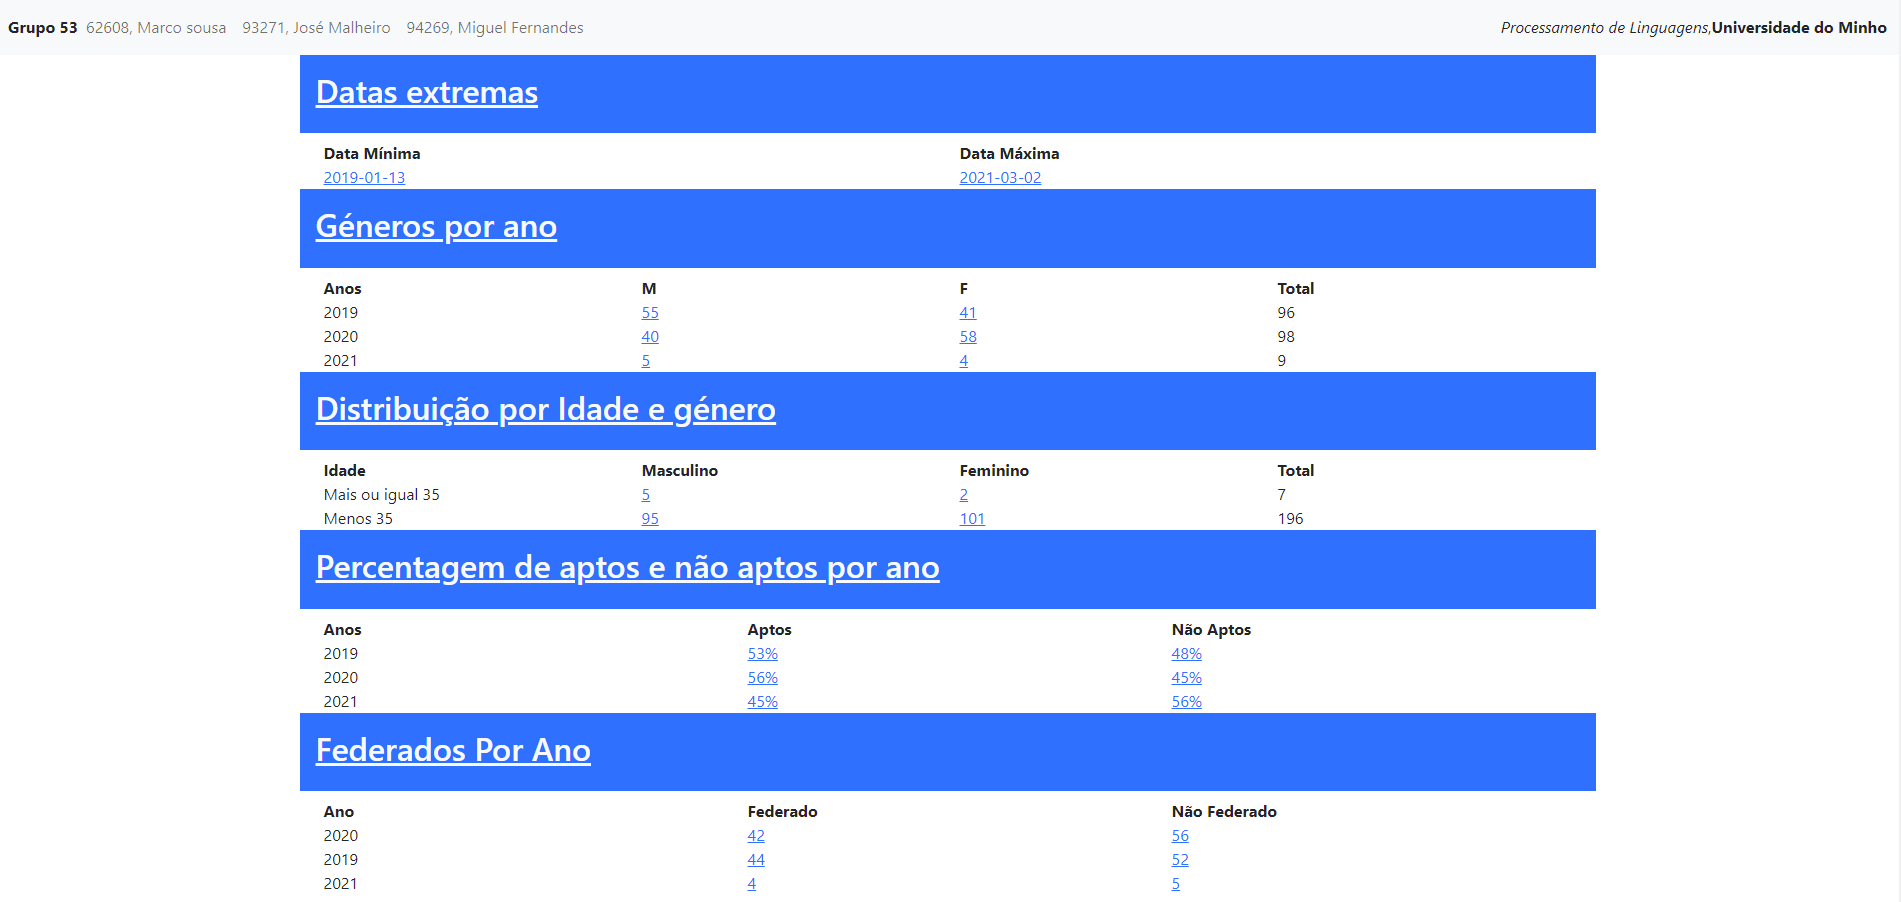
\includegraphics[width=\linewidth]{assets/index1.png}
    \caption{Ficheiro \textbf{index.html} - 1}
    \label{fig:index.html1}
\end{figure}

\begin{figure}
    \centering
    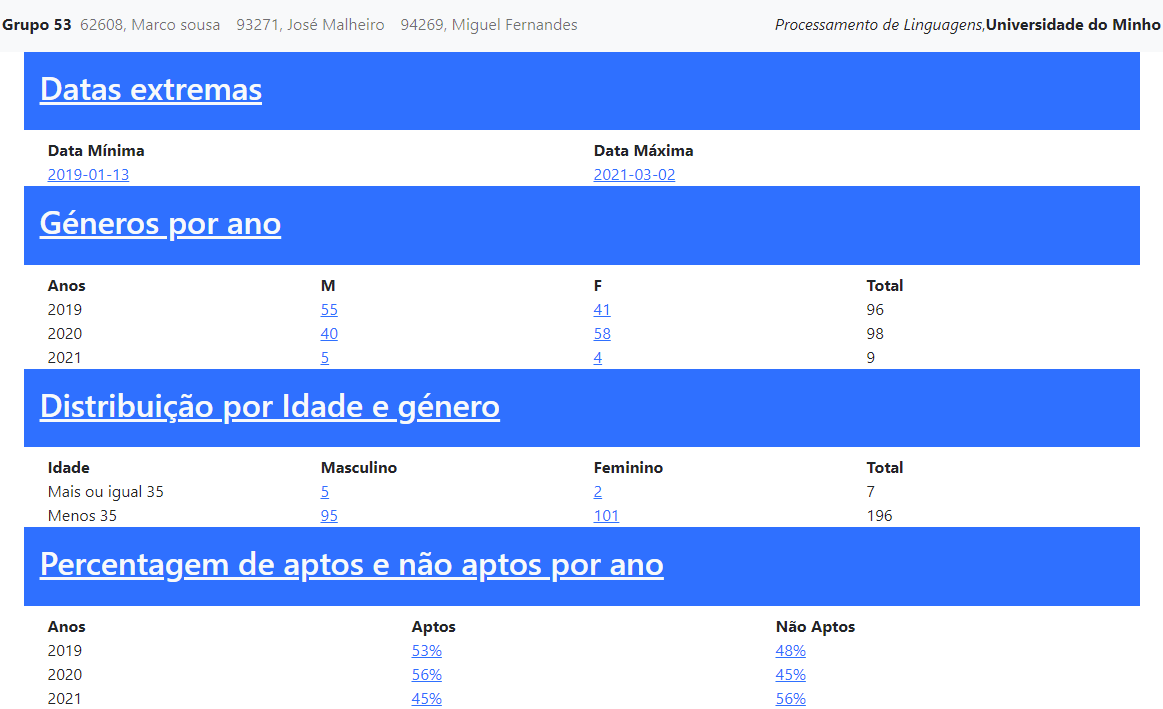
\includegraphics[width=\linewidth]{assets/index2.png}
    \caption{Ficheiro \textbf{index.html} - 2}
    \label{fig:index.html2}
\end{figure}

\begin{figure}
    \centering
    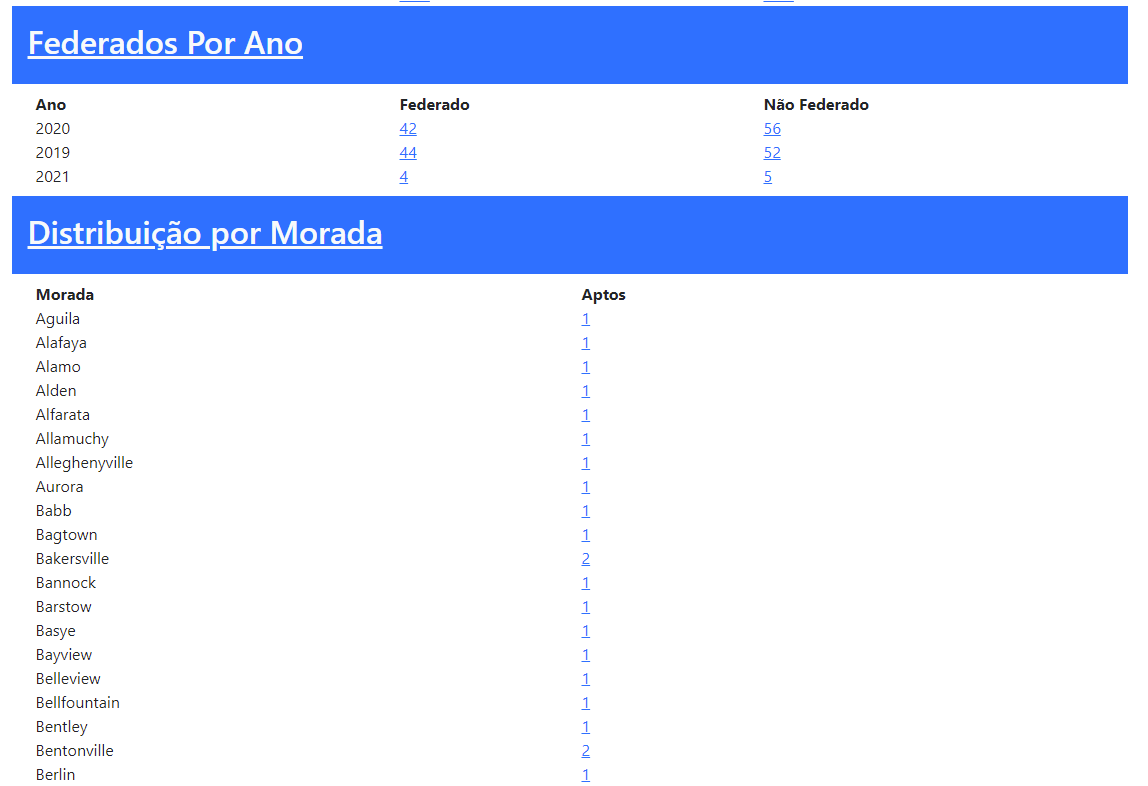
\includegraphics[width=\linewidth]{assets/index3.png}
    \caption{Ficheiro \textbf{index.html} - 3}
    \label{fig:index.html3}
\end{figure}

\begin{figure}
    \centering
    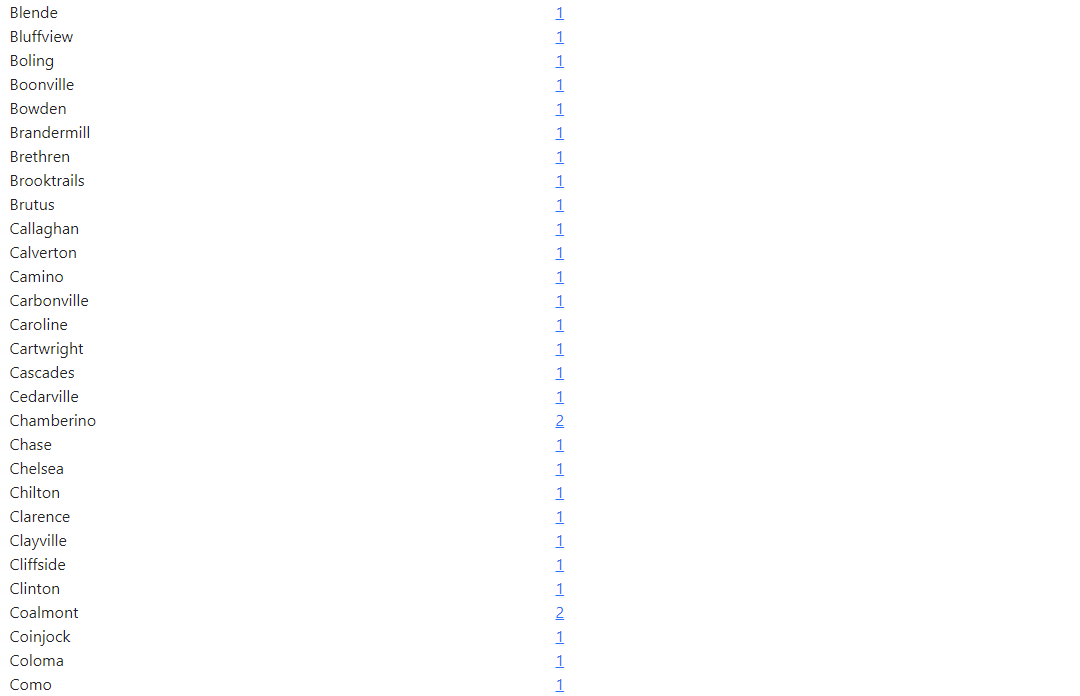
\includegraphics[width=\linewidth]{assets/index4.png}
    \caption{Ficheiro \textbf{index.html} - 4}
    \label{fig:index.html4}
\end{figure}

\begin{figure}
    \centering
    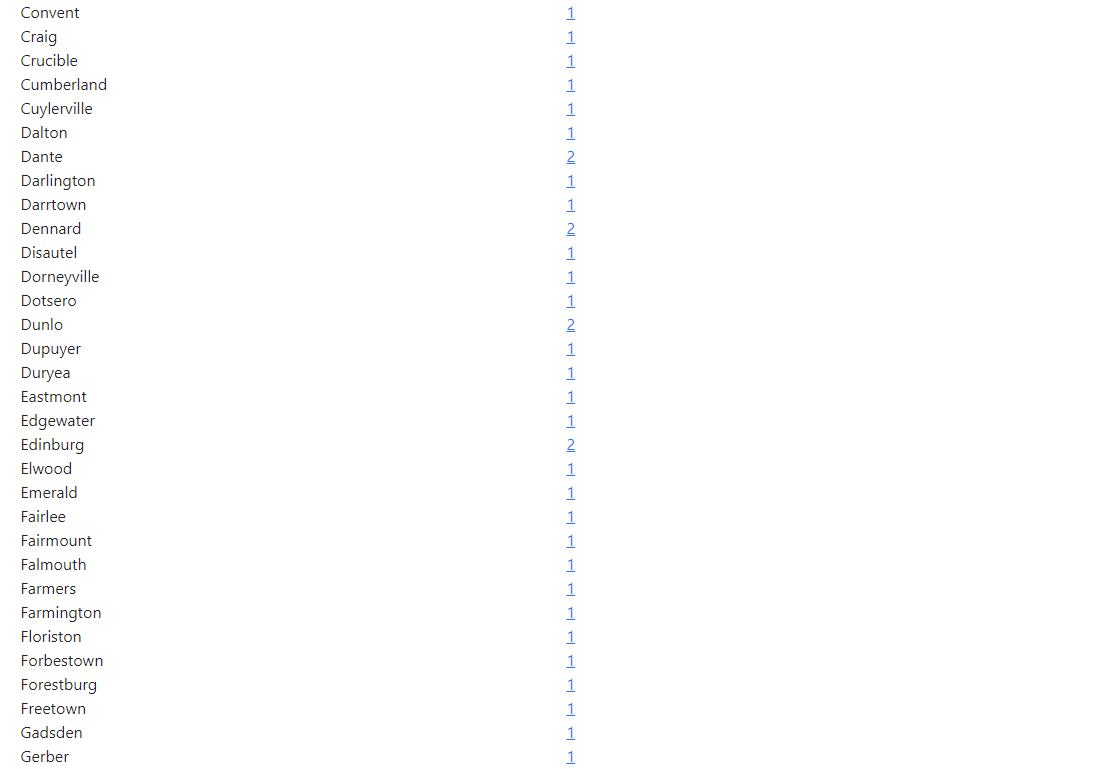
\includegraphics[width=\linewidth]{assets/index5.png}
    \caption{Ficheiro \textbf{index.html} - 5}
    \label{fig:index.html5}
\end{figure}

\begin{figure}
    \centering
    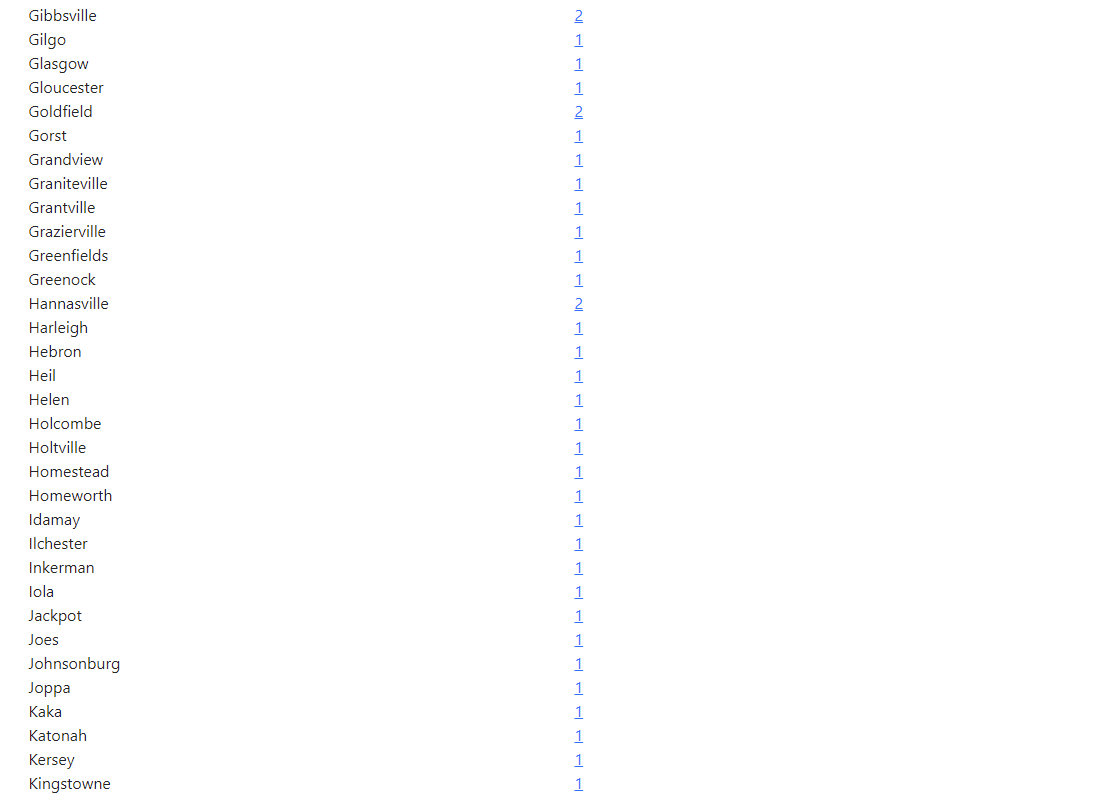
\includegraphics[width=\linewidth]{assets/index6.png}
    \caption{Ficheiro \textbf{index.html} - 6}
    \label{fig:index.html6}
\end{figure}

\begin{figure}
    \centering
    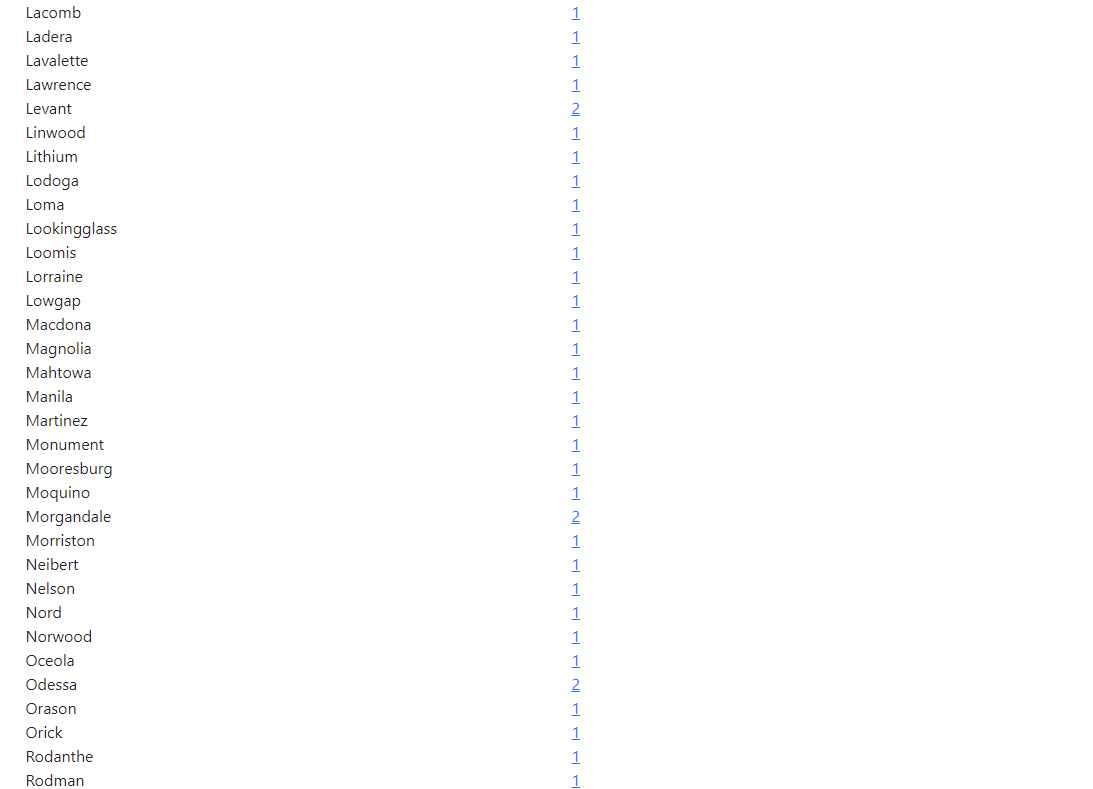
\includegraphics[width=\linewidth]{assets/index7.png}
    \caption{Ficheiro \textbf{index.html} - 7}
    \label{fig:index.html7}
\end{figure}


\begin{figure}
    \centering
    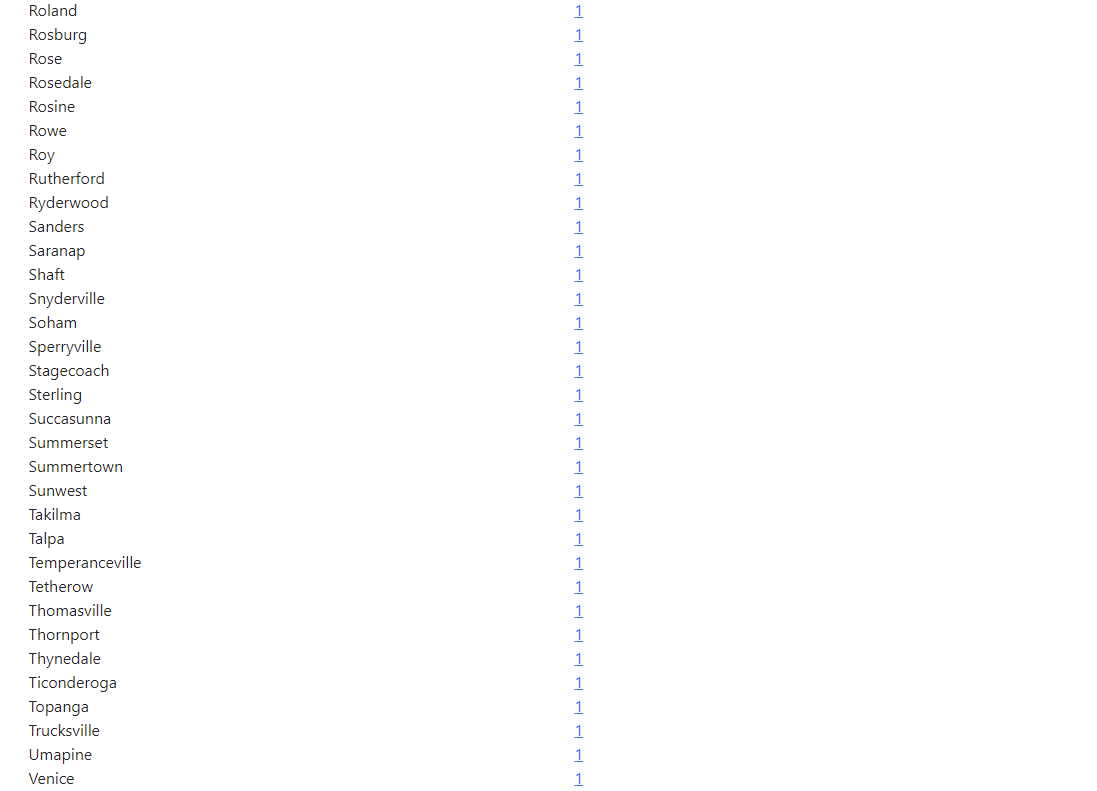
\includegraphics[width=\linewidth]{assets/index8.png}
    \caption{Ficheiro \textbf{index.html} - 8}
    \label{fig:index.html8}
\end{figure}


\begin{figure}
    \centering
    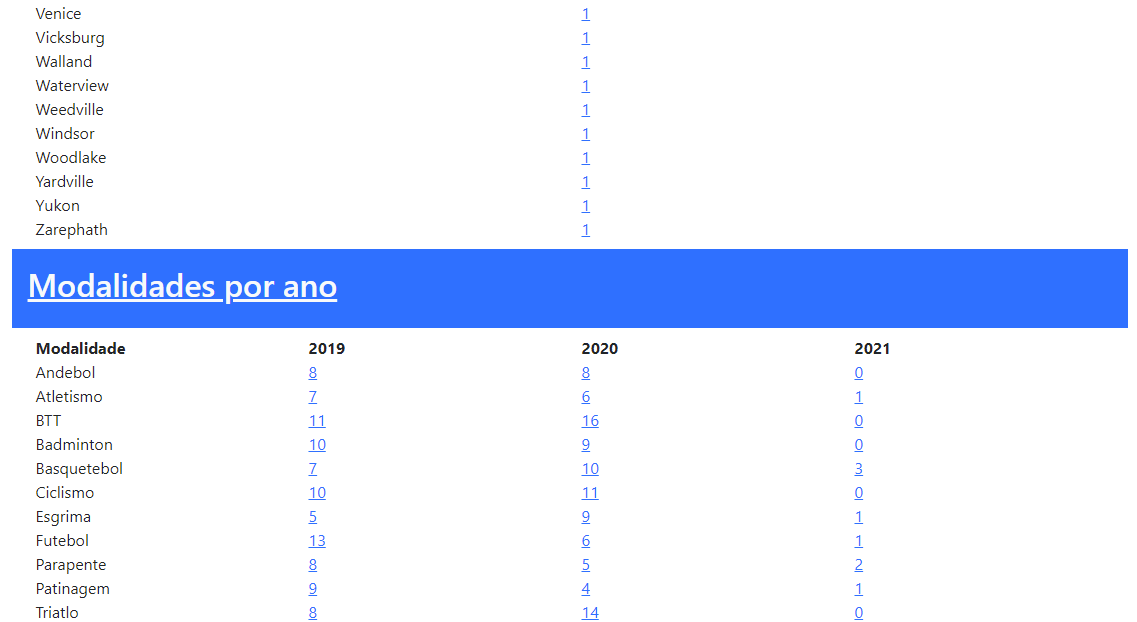
\includegraphics[width=\linewidth]{assets/index9.png}
    \caption{Ficheiro \textbf{index.html} - 9}
    \label{fig:index.html9}
\end{figure}

%
% ---- Bibliography ----
%
% BibTeX users should specify bibliography style 'splncs04'.
% References will then be sorted and formatted in the correct style.
%
% \bibliographystyle{splncs04}
% \bibliography{mybibliography}
% %
% \begin{thebibliography}{1}
% \bibitem{ref_article1}
% Author, F.: Article title. Journal \textbf{2}(5), 99--110 (2016)

% \bibitem{ref_lncs1}
% Author, F., Author, S.: Title of a proceedings paper. In: Editor,
% F., Editor, S. (eds.) CONFERENCE 2016, LNCS, vol. 9999, pp. 1--13.
% Springer, Heidelberg (2016). \doi{10.10007/1234567890}

% \end{thebibliography}

\end{document}